%% LyX 2.4.0~beta5 created this file.  For more info, see https://www.lyx.org/.
%% Do not edit unless you really know what you are doing.
\documentclass[english,footrule]{foils}
\usepackage[T1]{fontenc}
\usepackage[latin9]{inputenc}
\pagestyle{foilheadings}
\setcounter{secnumdepth}{1}
\setcounter{tocdepth}{1}
\usepackage{color}
\usepackage{pifont}
\usepackage{url}
\usepackage{amsmath}
\usepackage{amsthm}
\usepackage{amssymb}
\usepackage{graphicx}

\makeatletter
%%%%%%%%%%%%%%%%%%%%%%%%%%%%%% User specified LaTeX commands.
\newcommand{\argmin}{\operatornamewithlimits{argmin}}

\usepackage{xcolor}
\renewcommand{\labelitemi}{$\textcolor{blue}{\bullet}$}
\renewcommand{\labelitemii}{$\textcolor{teal}{\Rightarrow}$}
\renewcommand{\labelitemiii}{$\textcolor{red}{\rightarrow}$}
\renewcommand{\labelitemiv}{$\textcolor{brown}{\circ}$}

\newcommand{\T}{\mathrm{T}}  % transpose
\newcommand{\PP}{\mathrm{P}}  % probability
\newcommand{\dd}{\mathrm{d}} % integration dx
\newcommand{\ee}{\mathrm{e}} % exponential
\newcommand{\E}{\mathrm{E}} % expectation

%_%_%_%_%_%_%_%_
% for tikz drawings and cartoons
%_%_%_%_%_%_%_%_

\usepackage{tikz}

% for tikzit drawings
\usepackage{tikzit}
\input{flow.tikzstyles}


% for decision trees:
\tikzset{
	treenode/.style = {shape=rectangle, rounded corners,
		draw, align=center,
		top color=white, bottom color=blue!20},
	root/.style     = {treenode, font=\Large, bottom color=red!30},
	env0/.style     = {treenode, font=\large, bottom color=orange!30},
	env1/.style     = {treenode,  bottom color=green!30},
	env/.style      = {treenode, font=\ttfamily\normalsize},
    leaf/.style      = {treenode, font=\ttfamily\normalsize},
	dummy/.style    = {circle,draw}
}
\usetikzlibrary{positioning}

\makeatother

\usepackage{babel}
\begin{document}

\MyLogo{Intro ML--Neural Networks}
\title{Supervised Learning - Neural Networks (NN)}
\author{Mark Asch - IMU/VLP/CSU }
\date{2023}
\maketitle

\foilhead{Program}
\begin{enumerate}
\item Data Analysis

\begin{enumerate}
\item Introduction: the 4 identifiers of ``big data'' and ``data science''
\item \textcolor{red}{Supervised learning methods:} regression---advanced,
k-NN, linear classification methods, SVM, \textcolor{red}{NN}, decision
trees. 
\item Unsupervised learning methods: k-means, principal component analysis,
clustering.
\end{enumerate}
\end{enumerate}

\foilhead{Introduction}
\begin{itemize}
\item A neural network (NN) is a \textcolor{magenta}{supervised learning}
model for classification or regression, 
\begin{itemize}
\item We use the data/observations/measurements to train the NN. 
\item The NN learns a functional relation between inputs, $X,$ and outputs,
$Y.$ 
\item The NN in fact learns an approximation to the relation by iterative
fitting of its parameters. 
\end{itemize}
\item The simplest model of an NN is the \textcolor{magenta}{multilayer
perceptron} (MLP that has the impressive property of being a \textcolor{magenta}{universal
approximator-{}}-{}-see below. 
\begin{itemize}
\item It can be proved that MLPs, as universal approximators, can model
any suitable smooth function, given enough hidden units, to any desired
level of precision. 
\item These hidden units are made up of (linear combinations of) \textcolor{magenta}{nonlinear
activation} functions whose parameters are ``hidden'' from the model,
in that they are intermediary, unobserved variables in the model. 
\item The network is a\textcolor{magenta}{{} directed graph} with an architecture
made up of 
\begin{itemize}
\item layers, 
\item nodes (``neurons'') and 
\item activation functions. 
\end{itemize}
\end{itemize}
\item NNs can become extremely complex and they tend to \textcolor{magenta}{overfit}.
\item They must thus be handled with \textcolor{magenta}{extreme care},
but when they work, the results are amazing!
\end{itemize}

\foilhead{Structure}
\begin{itemize}
\item The NN seeks to learn a \textcolor{magenta}{mapping}, $f,$ from the
input layer, $\mathbf{x},$ into the output layer $\mathbf{y}=f(\mathbf{x}).$ 
\item A \textcolor{magenta}{layer} is defined as a set of neurons having
no connections between them. 
\begin{itemize}
\item one layer reads the \textcolor{magenta}{input} signals, with a single
neuron per input $x_{i},$ $i=1,\ldots,4$ 
\item the \textcolor{magenta}{output} layer provides the response of the
system, ${y},$
\item one or more \textcolor{magenta}{hidden} layers, between the two, perform
the approximation.
\end{itemize}
\item A \textcolor{magenta}{neuron} is a model of a biological neuron---it
receives input signals, computes a weighted sum of the inputs, applies
an activation function and finally produces an output.
\end{itemize}

\foilhead[-0.5in]{Neurons and Layers}

\begin{center}\index{neural networks (NN)!multi layer perceptron (MLP)|ffi}
\def\layersep{2.5cm}
\begin{tikzpicture}[shorten >=1pt,->,draw=black!50, node distance=\layersep]
\tikzstyle{every pin edge}=[<-,shorten <=1pt]
\tikzstyle{neuron}=[circle,fill=black!25,minimum size=17pt,inner sep=0pt]
\tikzstyle{input neuron}=[neuron, fill=green!50];
\tikzstyle{output neuron}=[neuron, fill=red!50];
\tikzstyle{hidden neuron}=[neuron, fill=blue!50];
\tikzstyle{annot} = [text width=4em, text centered]

% Draw the input layer nodes
\foreach \name / \y in {1,...,4}
% This is the same as writing \foreach \name / \y in {1/1,2/2,3/3,4/4}
\node[input neuron, pin=left:Input $x_{\y}$] (I-\name) at (0,-\y) {};

% Draw the hidden layer nodes
\foreach \name / \y in {1,...,5}
\path[yshift=0.5cm]
node[hidden neuron] (H-\name) at (\layersep,-\y cm) {};

% Draw the output layer node
\node[output neuron,pin={[pin edge={->}]right:Output $y$}, right of=H-3] (O) {};

% Connect every node in the input layer with every node in the
% hidden layer.
\foreach \source in {1,...,4}
\foreach \dest in {1,...,5}
\path (I-\source) edge (H-\dest);

% Connect every node in the hidden layer with the output layer
\foreach \source in {1,...,5}
\path (H-\source) edge (O);

% Annotate the layers
\node[annot,above of=H-1, node distance=2cm] (hl) {Hidden layer};
\node[annot,left of=hl] {Input layer};
\node[annot,right of=hl] {Output layer};
\end{tikzpicture}
\end{center}

\begin{figure}
\begin{centering}
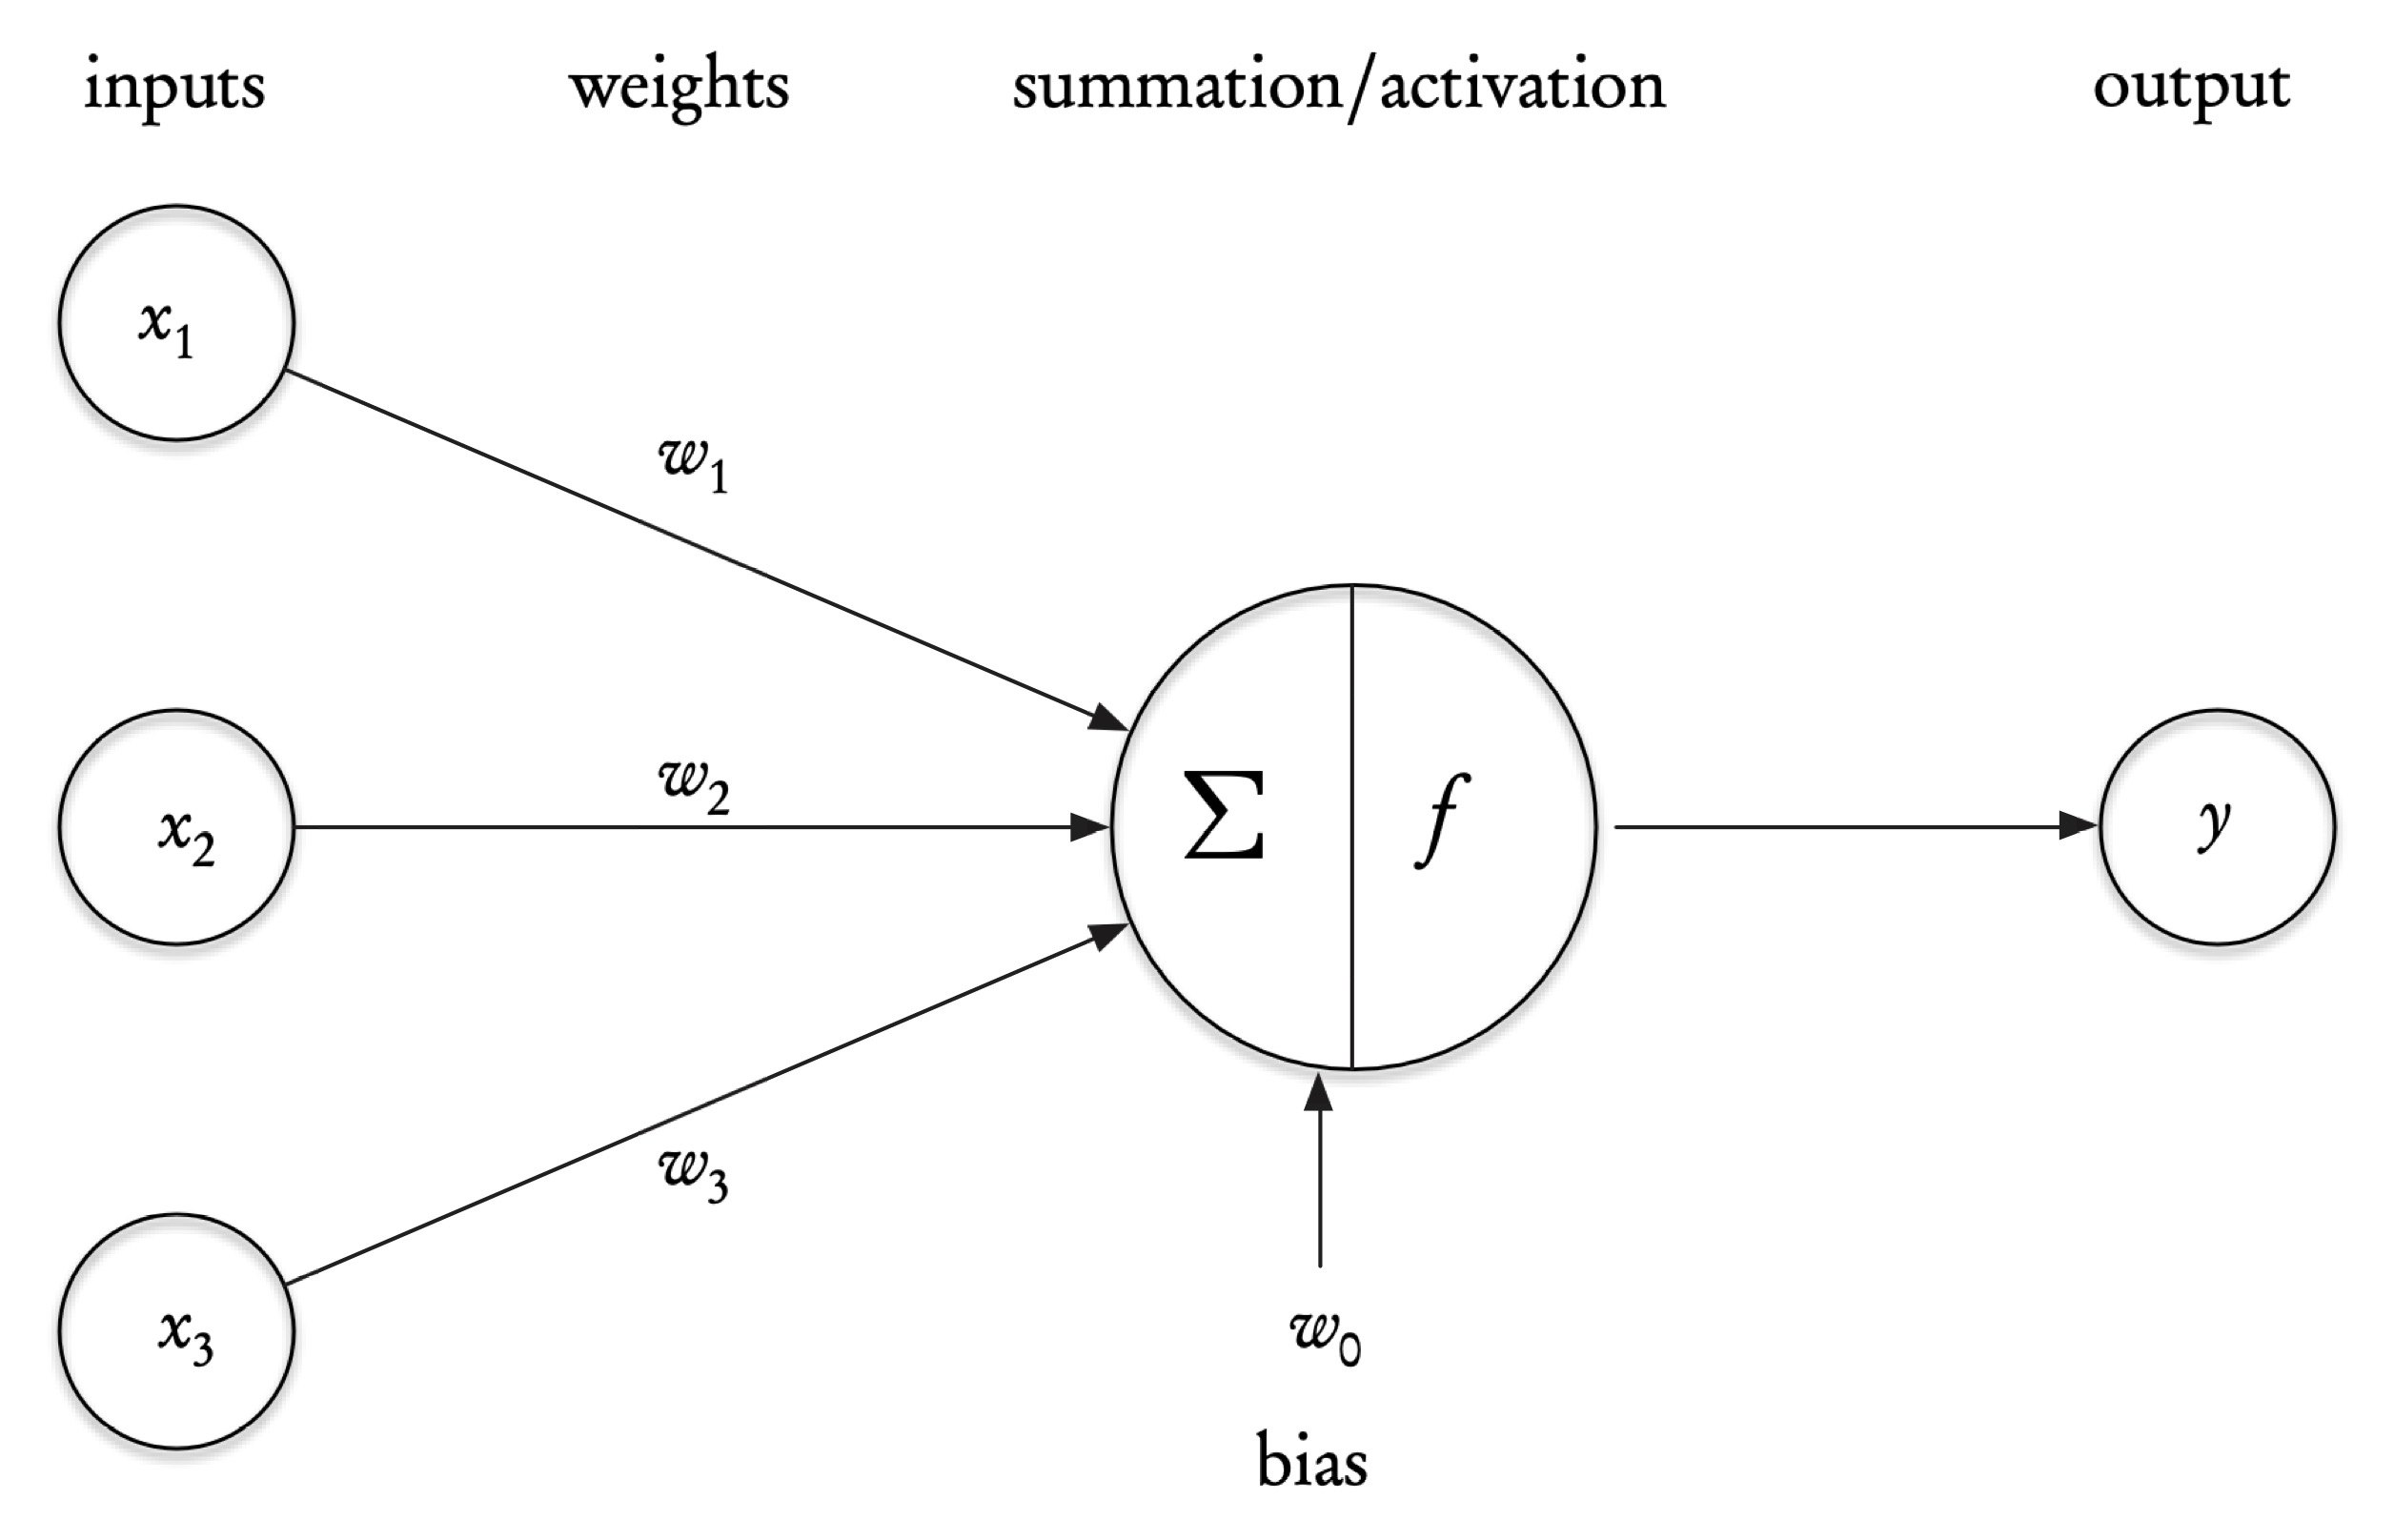
\includegraphics[scale=0.5]{/Users/markasch/Dropbox/6Books/DTbook/src/bwgraphics/neuron}
\par\end{centering}
\caption{A single neuron with output $y=f\left(w_{0}+\sum_{i=1}^{3}w_{i}x_{i}\right)$}
\end{figure}


\foilhead[-0.5in]{Networks with several layers}
\begin{itemize}
\item For simplicity, suppose that we have a\textcolor{magenta}{{} linear}
mapping between the layers, then $\mathbf{x}^{(1)}=A_{1}\mathbf{x},$
and ${y}=A_{2}\mathbf{x}^{(1).}$ 
\item The overall structure is then a \textcolor{magenta}{composition} of
linear operators ${y}=A_{2}A_{1}\mathbf{x}.$ 
\item This can be generalized to $M$ nonlinear mappings, and to a vector
output, 
\[
\mathbf{y}=f_{M}\left(A_{M},\dots,f_{2}(A_{2},f_{1}(A_{1}\mathbf{x}))\cdots\right).
\]
\end{itemize}
\begin{figure}
\begin{centering}
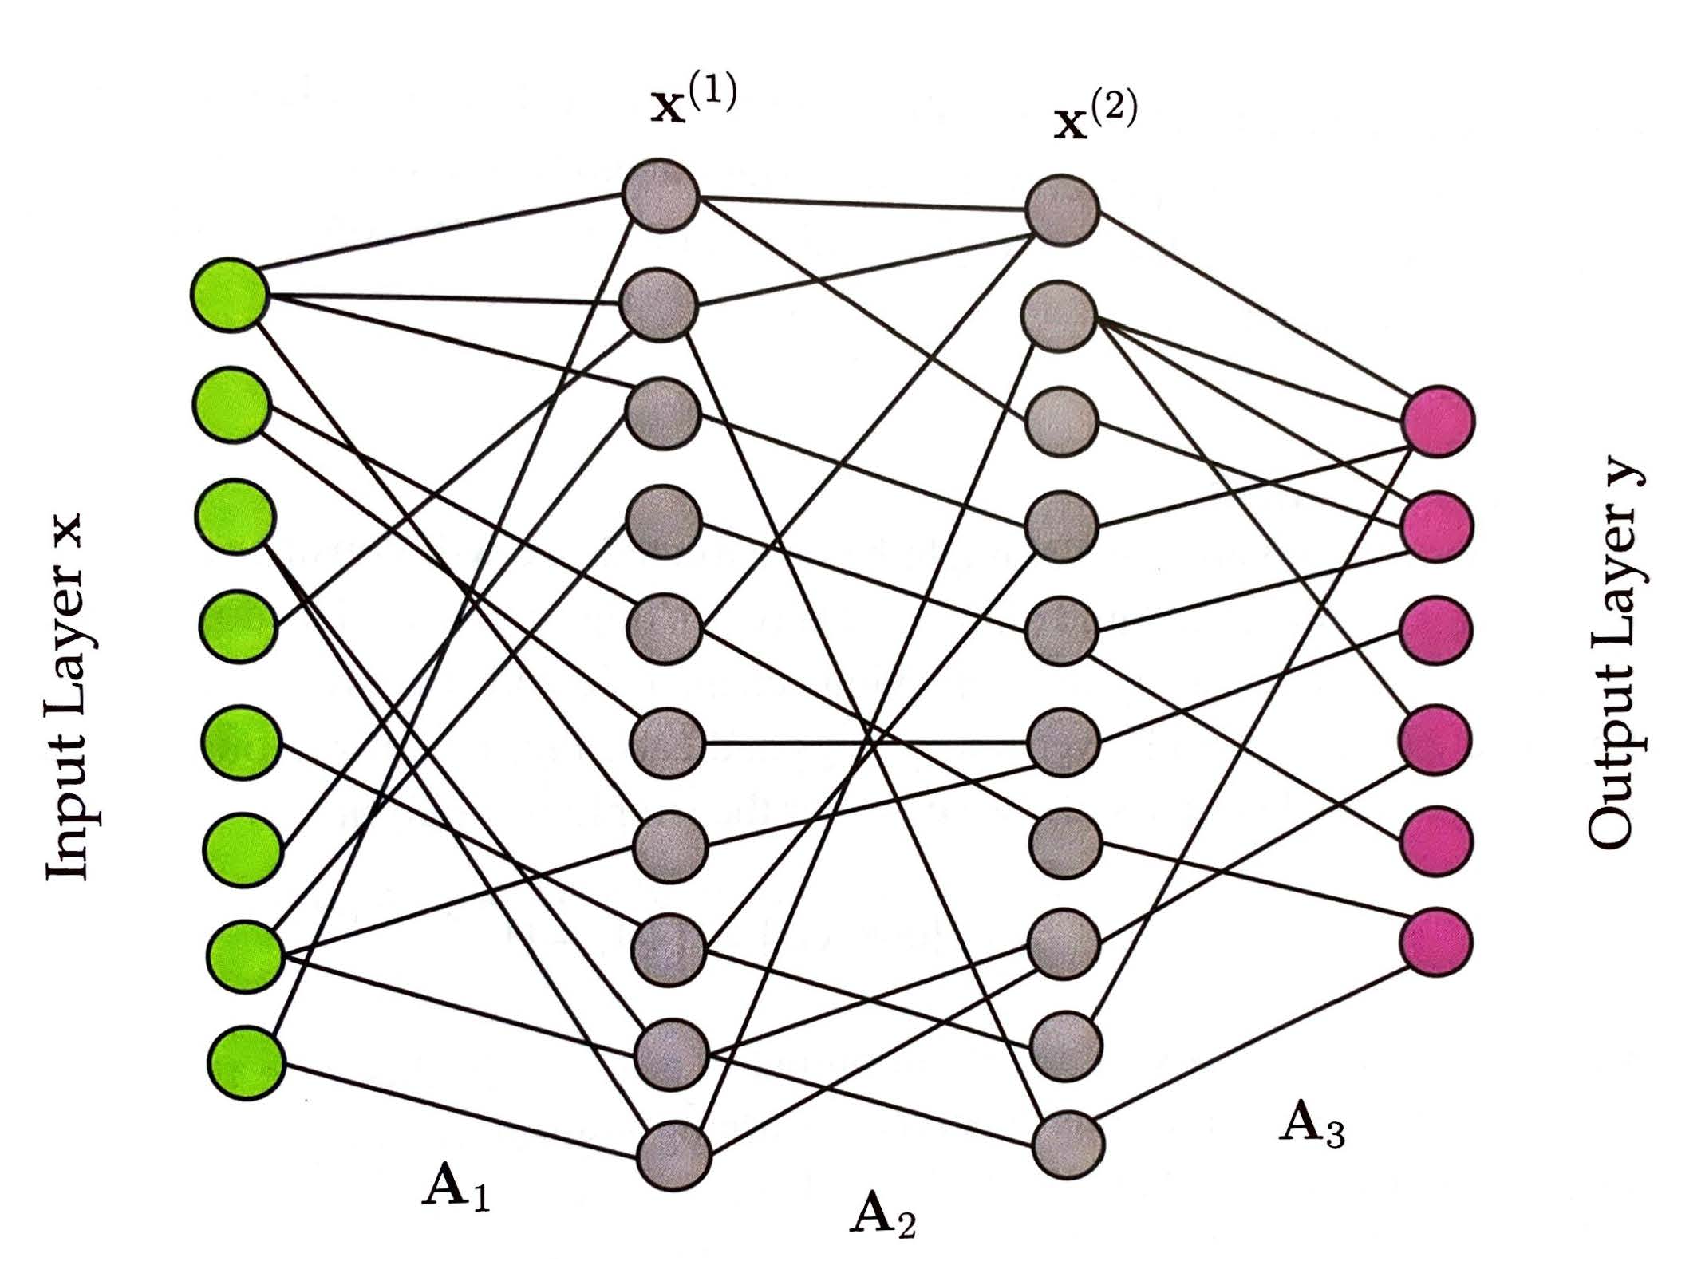
\includegraphics[scale=0.35]{graphics/nn-multilayer}
\par\end{centering}
\caption{Neural network with 2 hidden layers.}
\end{figure}


\foilhead{Formulation}
\begin{itemize}
\item Then, as in all the rest of ML, the objective is to find the unknown
model parameters by \textcolor{magenta}{optimizing}. In this case,
the system is highly under-determined (there are far fewer equations
than unknowns) and some type of regularization will be necessary. 
\item The problem then is to compute 
\[
\argmin_{A_{j}}\left[f_{M}\left(A_{M},\dots,f_{2}(A_{2},f_{1}(A_{1}\mathbf{x}))\cdots\right)+\lambda g(A_{j})\right],
\]
which is an underdetermined system regularized by $\lambda g(A_{j}),$
where $\lambda$ is a regularization coefficient and $g$ is a smoothing
function.
\item This is usually performed by a \textcolor{magenta}{stochastic gradient}
plus \textcolor{magenta}{backpropagation} algorithm (see Advanced
Course). 
\item This should, as always, be followed systematically by \textcolor{magenta}{cross
validation}.
\end{itemize}

\foilhead{Activation Functions}
\begin{itemize}
\item In the sought for mapping from input to output space, we will write
\[
\mathbf{y}=f(\mathbf{A,x})
\]
and $f$ will be called the \textcolor{magenta}{activation function},
borrowing from the neuroscience analogy. 
\item \textcolor{magenta}{Nonlinear} activation functions are used, since
linear mappings (even composed) can only provide a limited range of
functional responses. 
\item The principal ones are, 
\begin{align*}
f(x) & =x,\quad\mathrm{linear},\\
f(x) & =\mathbf{1}_{0,+\infty}(x),\quad\mathrm{threshold},\\
f(x) & =\begin{cases}
0, & x\le0\\
x, & x>0,
\end{cases}\quad\mathrm{ReLU},\\
f(x) & =\tanh(x),\quad\mathrm{hyperbolic\;tangent},\\
f(x) & =1/(1+e^{-x}),\quad\mathrm{soft\,step.}
\end{align*}
\item The function $f$ performs a transformation of an affine combination
of input signals 
\[
\mathbf{y}=f(\mathbf{x})=f(\alpha_{0}+\boldsymbol{\alpha}^{\T}\mathbf{x}),
\]
where $\alpha_{0}$ is the \textcolor{magenta}{bias} of the neuron,
$\boldsymbol{\alpha}=\left[\alpha_{1},\ldots,\alpha_{p}\right]^{\T}$
is a vector of \textcolor{magenta}{weights} associated to each neuron. 
\begin{itemize}
\item These are the values that are estimated in the training phase and
they constitute the ``memory'', or distributed knowledge of the
network. 
\item The two most commonly used activation functions are the\textcolor{magenta}{{}
Rectified Linear Unit (ReLU),} the \textcolor{magenta}{sigmoid (soft-step)}
and the \textcolor{magenta}{hyperbolic tangent (tanh)}.
\end{itemize}
\end{itemize}

\foilhead{Training}
\begin{itemize}
\item The basis for the learning phase is made up of 
\begin{itemize}
\item the $n$ \textcolor{magenta}{observations} $\left\{ x_{i}^{1},\ldots,x_{i}^{p};y_{i}\right\} _{i=1}^{n},$ 
\item the $p$ \textcolor{magenta}{explanatory} variables (covariates) $X^{1},\ldots,X^{p}$
and
\item the (\textcolor{magenta}{response}) variable to be predicted $Y.$ 
\end{itemize}
\item Let us consider, as a simple example, the case of regression with
a network made up of one neuron with linear output and a hidden layer
of $q$ neurons whose parameters will be computed by \textcolor{magenta}{minimization}
of the least squares criterion (\textcolor{magenta}{loss function})
\[
Q(\alpha,\beta)=\sum_{i=1}^{n}\left[y_{i}-f(x;\alpha,\beta\right]^{2},
\]
where $\beta$ are the regression coefficients
\item This minimization is usually performed by variants of stochastic gradient
with backpropagation---see the Advanced Course for details.
\end{itemize}

\foilhead{Choice of Parameters}

To perform this training, the user must follow these steps: 
\begin{enumerate}
\item \textcolor{magenta}{Input} and \textcolor{magenta}{output} variables
must, as in most statistical treatments, be transformed, centered
and \textcolor{magenta}{scaled} to avoid too large disparities and
over sensitivity to small errors in the estimation process. 
\item Network \textcolor{magenta}{architecture} must be designed: 
\begin{enumerate}
\item Choose the \textcolor{magenta}{number of hidden layers} that will
determine the aptitude of the network to deal with nonlinearity. 
\item Choose the \textcolor{magenta}{number of neurons} per hidden layer. 
\item These two choices will directly condition the number of parameters
(\textcolor{magenta}{weights}) to estimate and thus the\textcolor{magenta}{{}
model complexity}. They contribute to the search for a reasonable
\textcolor{magenta}{compromise} between \textcolor{magenta}{bias and
variance} that determines the balance between training quality and
forecast quality. 
\end{enumerate}
\item Three additional parameters influence the above compromise: 
\begin{enumerate}
\item the maximum number of \textcolor{magenta}{iterations}, 
\item the maximum \textcolor{magenta}{error tolerance}, and 
\item an eventual \textcolor{magenta}{regularization} term for ridge decay
(to eliminate terms with``weak'' influence on the parameters---see
previous lecture on Regression.)
\end{enumerate}
\item Choose the \textcolor{magenta}{training/learning rate }or the stochastic
gradient as well as an evolution strategy for it---see Advanced Course. 
\item Choose the size of the sets, or \textcolor{magenta}{batches}, of observations
that are to be considered at each iteration. 
\end{enumerate}
\begin{itemize}
\item In practice, all of these parameters cannot be tuned simultaneously
by the user. One has to, in priority, make choices regarding the control
of overtraining, or \textcolor{magenta}{overfitting}, by
\begin{itemize}
\item limiting the number of neurons, or the duration of the training, 
\item or increasing the penalization of the magnitude of these parameters. 
\end{itemize}
\item To do this, one needs to fix a method for estimating the error, by
using either 
\begin{itemize}
\item a \textcolor{magenta}{validation} sample, 
\item or a form of \textcolor{magenta}{cross validation} (including bootstrapping). 
\end{itemize}
\item A simple, but efficient strategy is to introduce a relatively large
number of neurons, then optimize the unique regularization (decay)
parameter by cross-validation. These important issues of tuning and
cross-validation will be discussed in a dedicated lecture.
\end{itemize}

\foilhead{Universal Approximation Property}
\begin{itemize}
\item The reason, at least theoretically, why neural networks can be so
effective are their \textcolor{magenta}{universal approximation }properties. 
\item These theoretical results {[}Pinkus,1999{]} show that any functional
relationship, $f,$ can be approximated, to within a desired tolerance,
by a neural network of sufficient depth (number of hidden layers)
and width (number of nodes in a layer). 
\item A very nice visual proof can be found at \textcolor{blue}{\url{http://neuralnetworksanddeeplearning.com/chap4.html}}.
\end{itemize}

\foilhead{Pros and Cons}
\begin{dinglist}{52}
\item The \textcolor{blue}{domains of application} of MLPs are numerous.
They cover discriminants, forecasting of time series, shape recognition,
and many others. These are generally well explained in the documentation
of the specialized software packages.
\end{dinglist}
\begin{dinglist}{56}
\item The \textcolor{magenta}{main criticisms} expressed, concern the difficulties
related to the training (computing time, sample size, local minima)
and the ``black box'' status of neural networks, in general. In fact,
contrary to discriminant or tree models, it is impossible to know
the effective influence of an input variable on the system as soon
as a hidden layer intervenes. Nonetheless, search techniques for system
sensitivity to each input can enable a focusing of the model and eventually
a simplification of the system by suppressing certain inputs. This
feature selection is often necessary.
\end{dinglist}
\begin{dinglist}{52}
\item On the other hand, MLPs have undeniable \textcolor{magenta}{qualities}
when there is no linearity and when the absence of explanatory variables
makes traditional statistical models ineffective or unusable. The
flexibility of NNs, thanks to the possibility of inserting specific
layers (especially in deep learning{[}Goodfellow2016{]}, coupled with
a training process that integrates weighting and choice of both variables
and their interactions, can make these networks extremely effective.
\end{dinglist}
\begin{dinglist}{56}
\item The downside of this flexibility is the risk, and the general tendency,
of neural network to \textcolor{magenta}{overfit} the data. As a result
the statistical models produced are often very brittle and suffer
from a lack of \textcolor{magenta}{explainability}, or interpretability.
\end{dinglist}

\foilhead{Other NNs}

\begin{figure}
\centering{}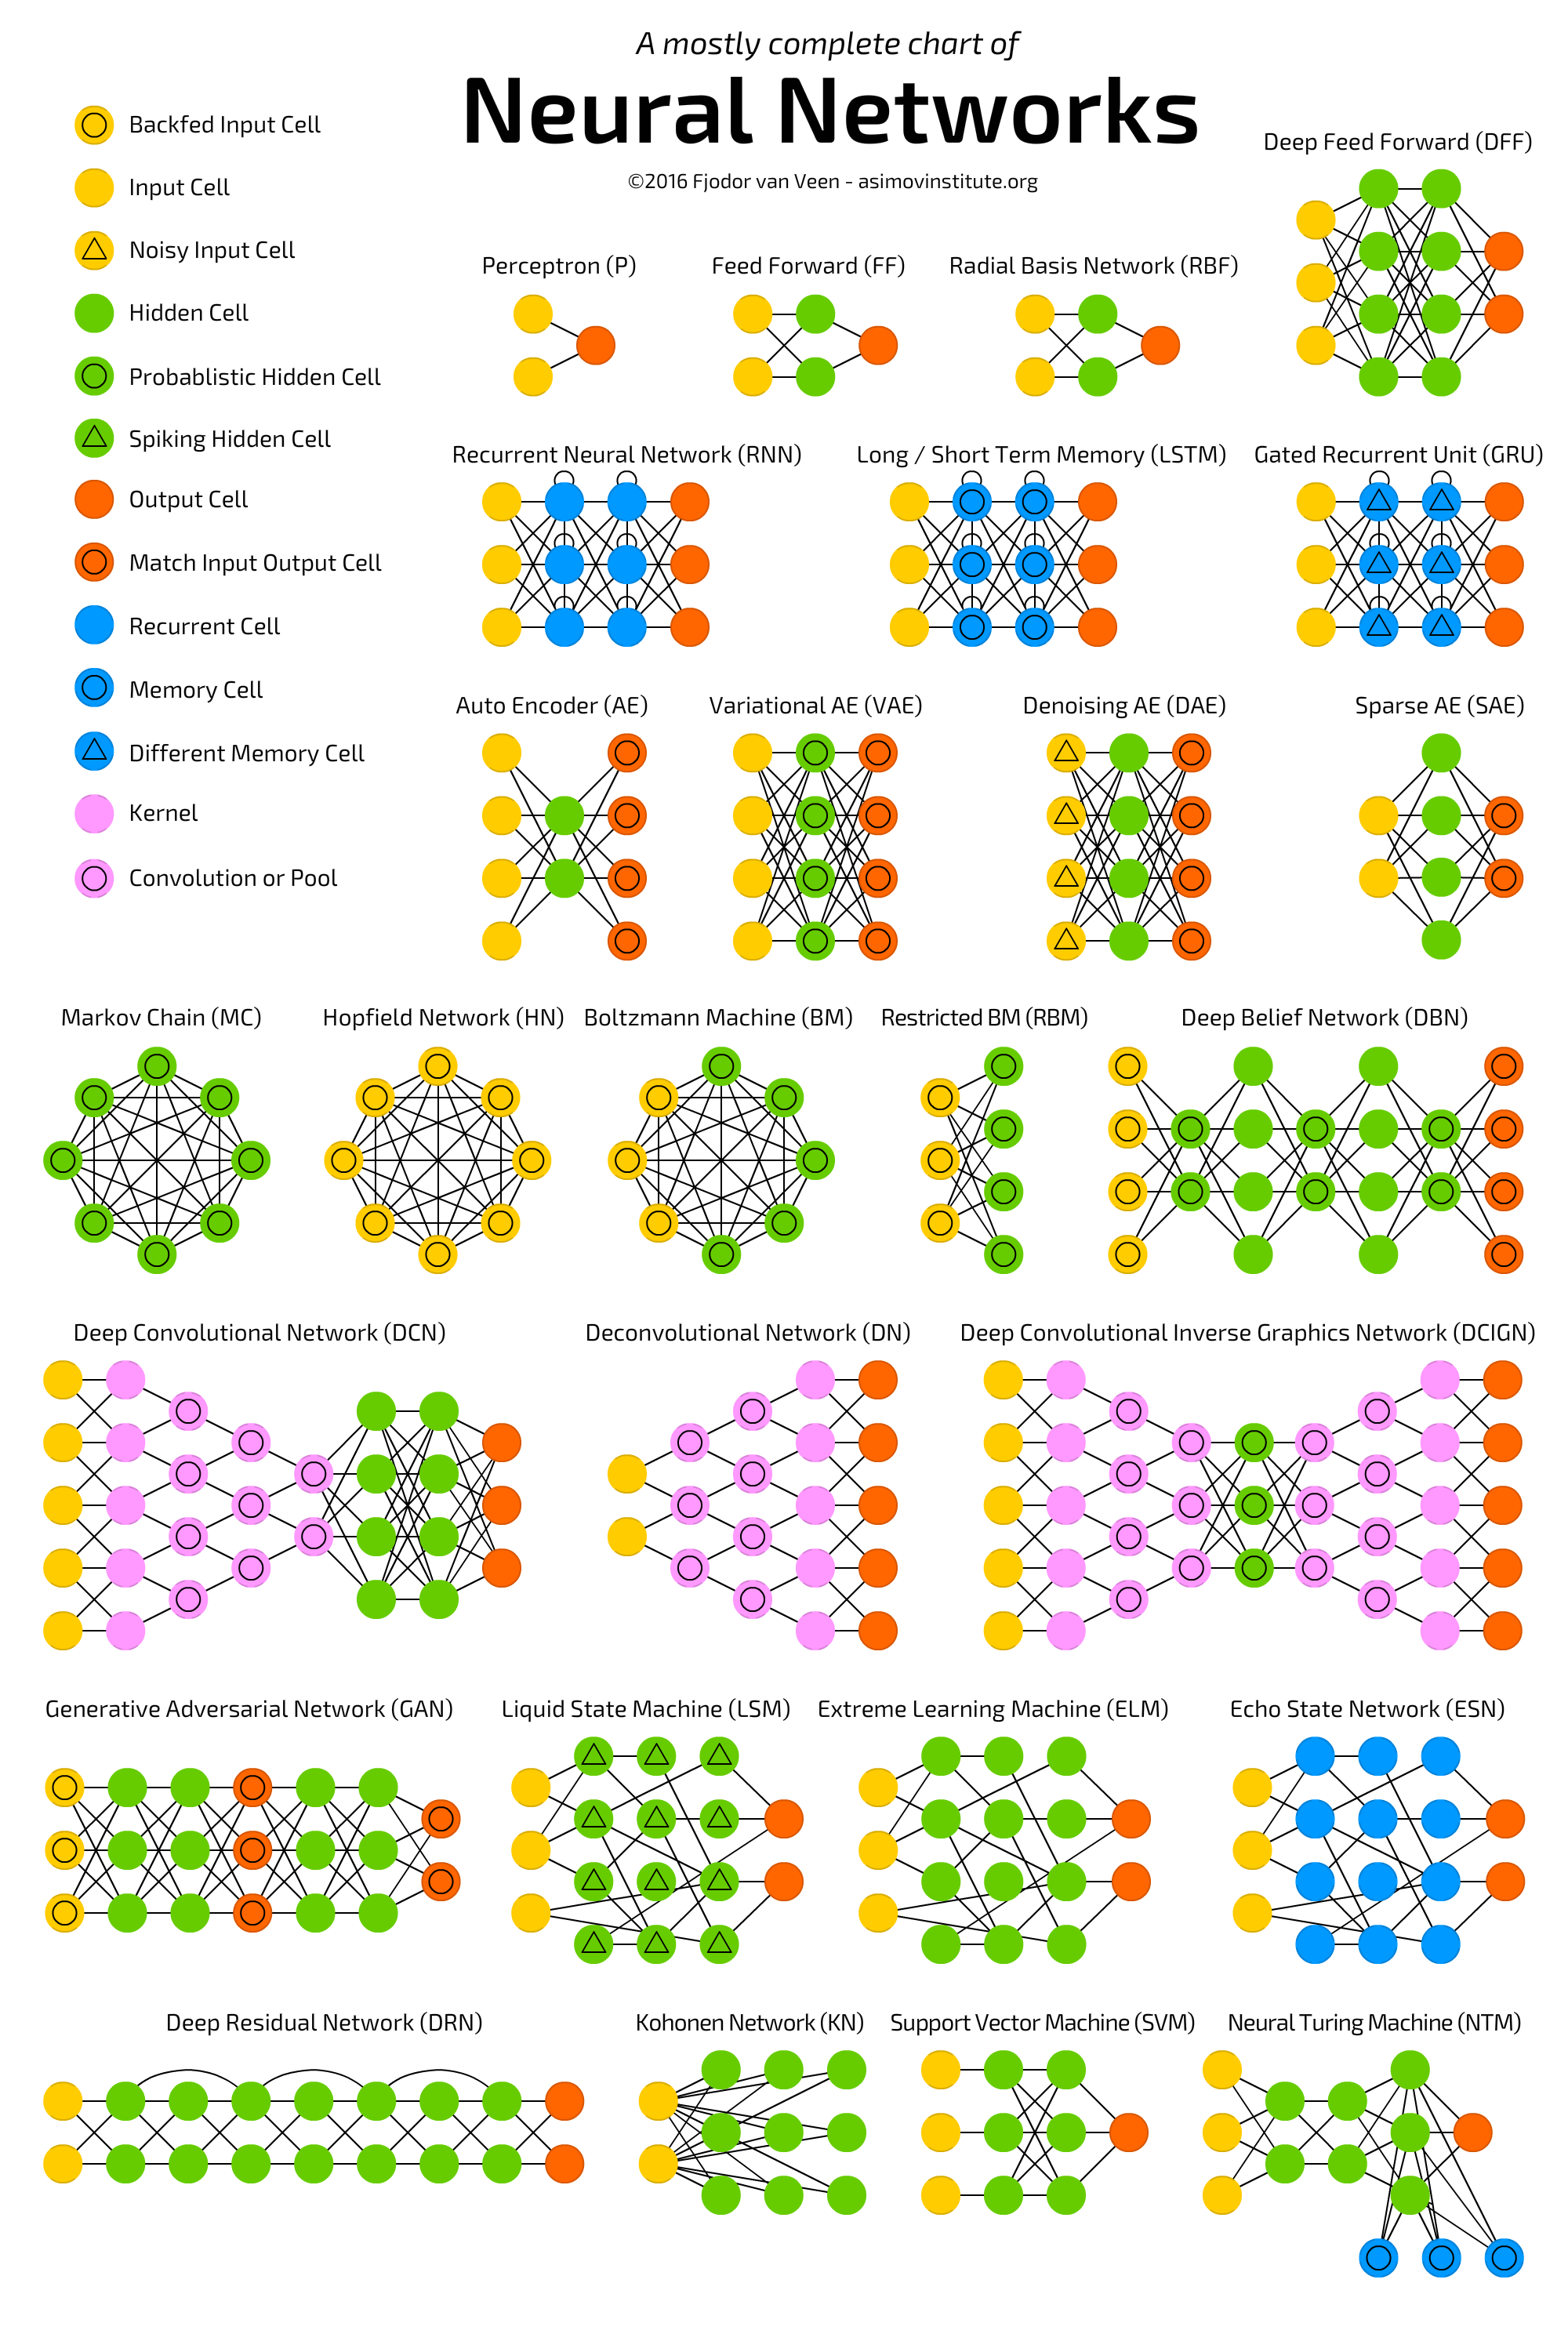
\includegraphics[scale=0.16]{graphics/nn-types}
\end{figure}

\begin{itemize}
\item Perceptrons (mulit-layer), fully-connected, feed-forward - the basis...
\item Convolutional Networks (CNN) - LeCun, image recognition
\item Recurrent Networks (RNN) - generalization of MLP
\item LSTM (long short term memory) - for time series
\item Hopfield Networks - dynamical systems
\item Boltzmann Machines - stochastic networks
\item Autoencodeurs - unsupervised training, similar to PCA
\item GAN (adversarial networks) - combination of 2 networks (generative,
discriminative)
\item Transformers - basis of LLMs (ChatGPT)
\end{itemize}

\foilhead{MLP 1: structure}
\begin{itemize}
\item MLPs can be applied to modeling any functional relationship thanks
to the ``\textcolor{magenta}{universal approximator}'' property
of these neural networks. 
\item The MLP is structured as a directed graph\footnote{We also encounter these in Bayesian networks and causality analysis.}
made up of \textcolor{magenta}{nodes} (or ``neurons'') and directed
\textcolor{magenta}{arcs} (the ``synapses''). 
\item The neurons, as shown above, are organized into \textcolor{magenta}{layers}
that are \textcolor{magenta}{completely connected} by the synapses
between two layers, but not within the layer.
\item As seen above, there are three types of layers:
\begin{itemize}
\item \textcolor{magenta}{Input layer} made up of all the covariates, each
in a separate neuron. 
\item \textcolor{magenta}{Output layer }made up of all the response variables. 
\item \textcolor{magenta}{Hidden layers} made up of an arbitrary number
of neurons. 
\end{itemize}
\item Note that the input and hidden layers contain a\textcolor{magenta}{{}
constant neuron} that is not influenced by (connected to) the covariates.
This neuron plays the role of the \textcolor{magenta}{bias}, or constant
term in the regression.
\end{itemize}

\foilhead{MLP 2: single-layer example}

\begin{figure}
\begin{centering}
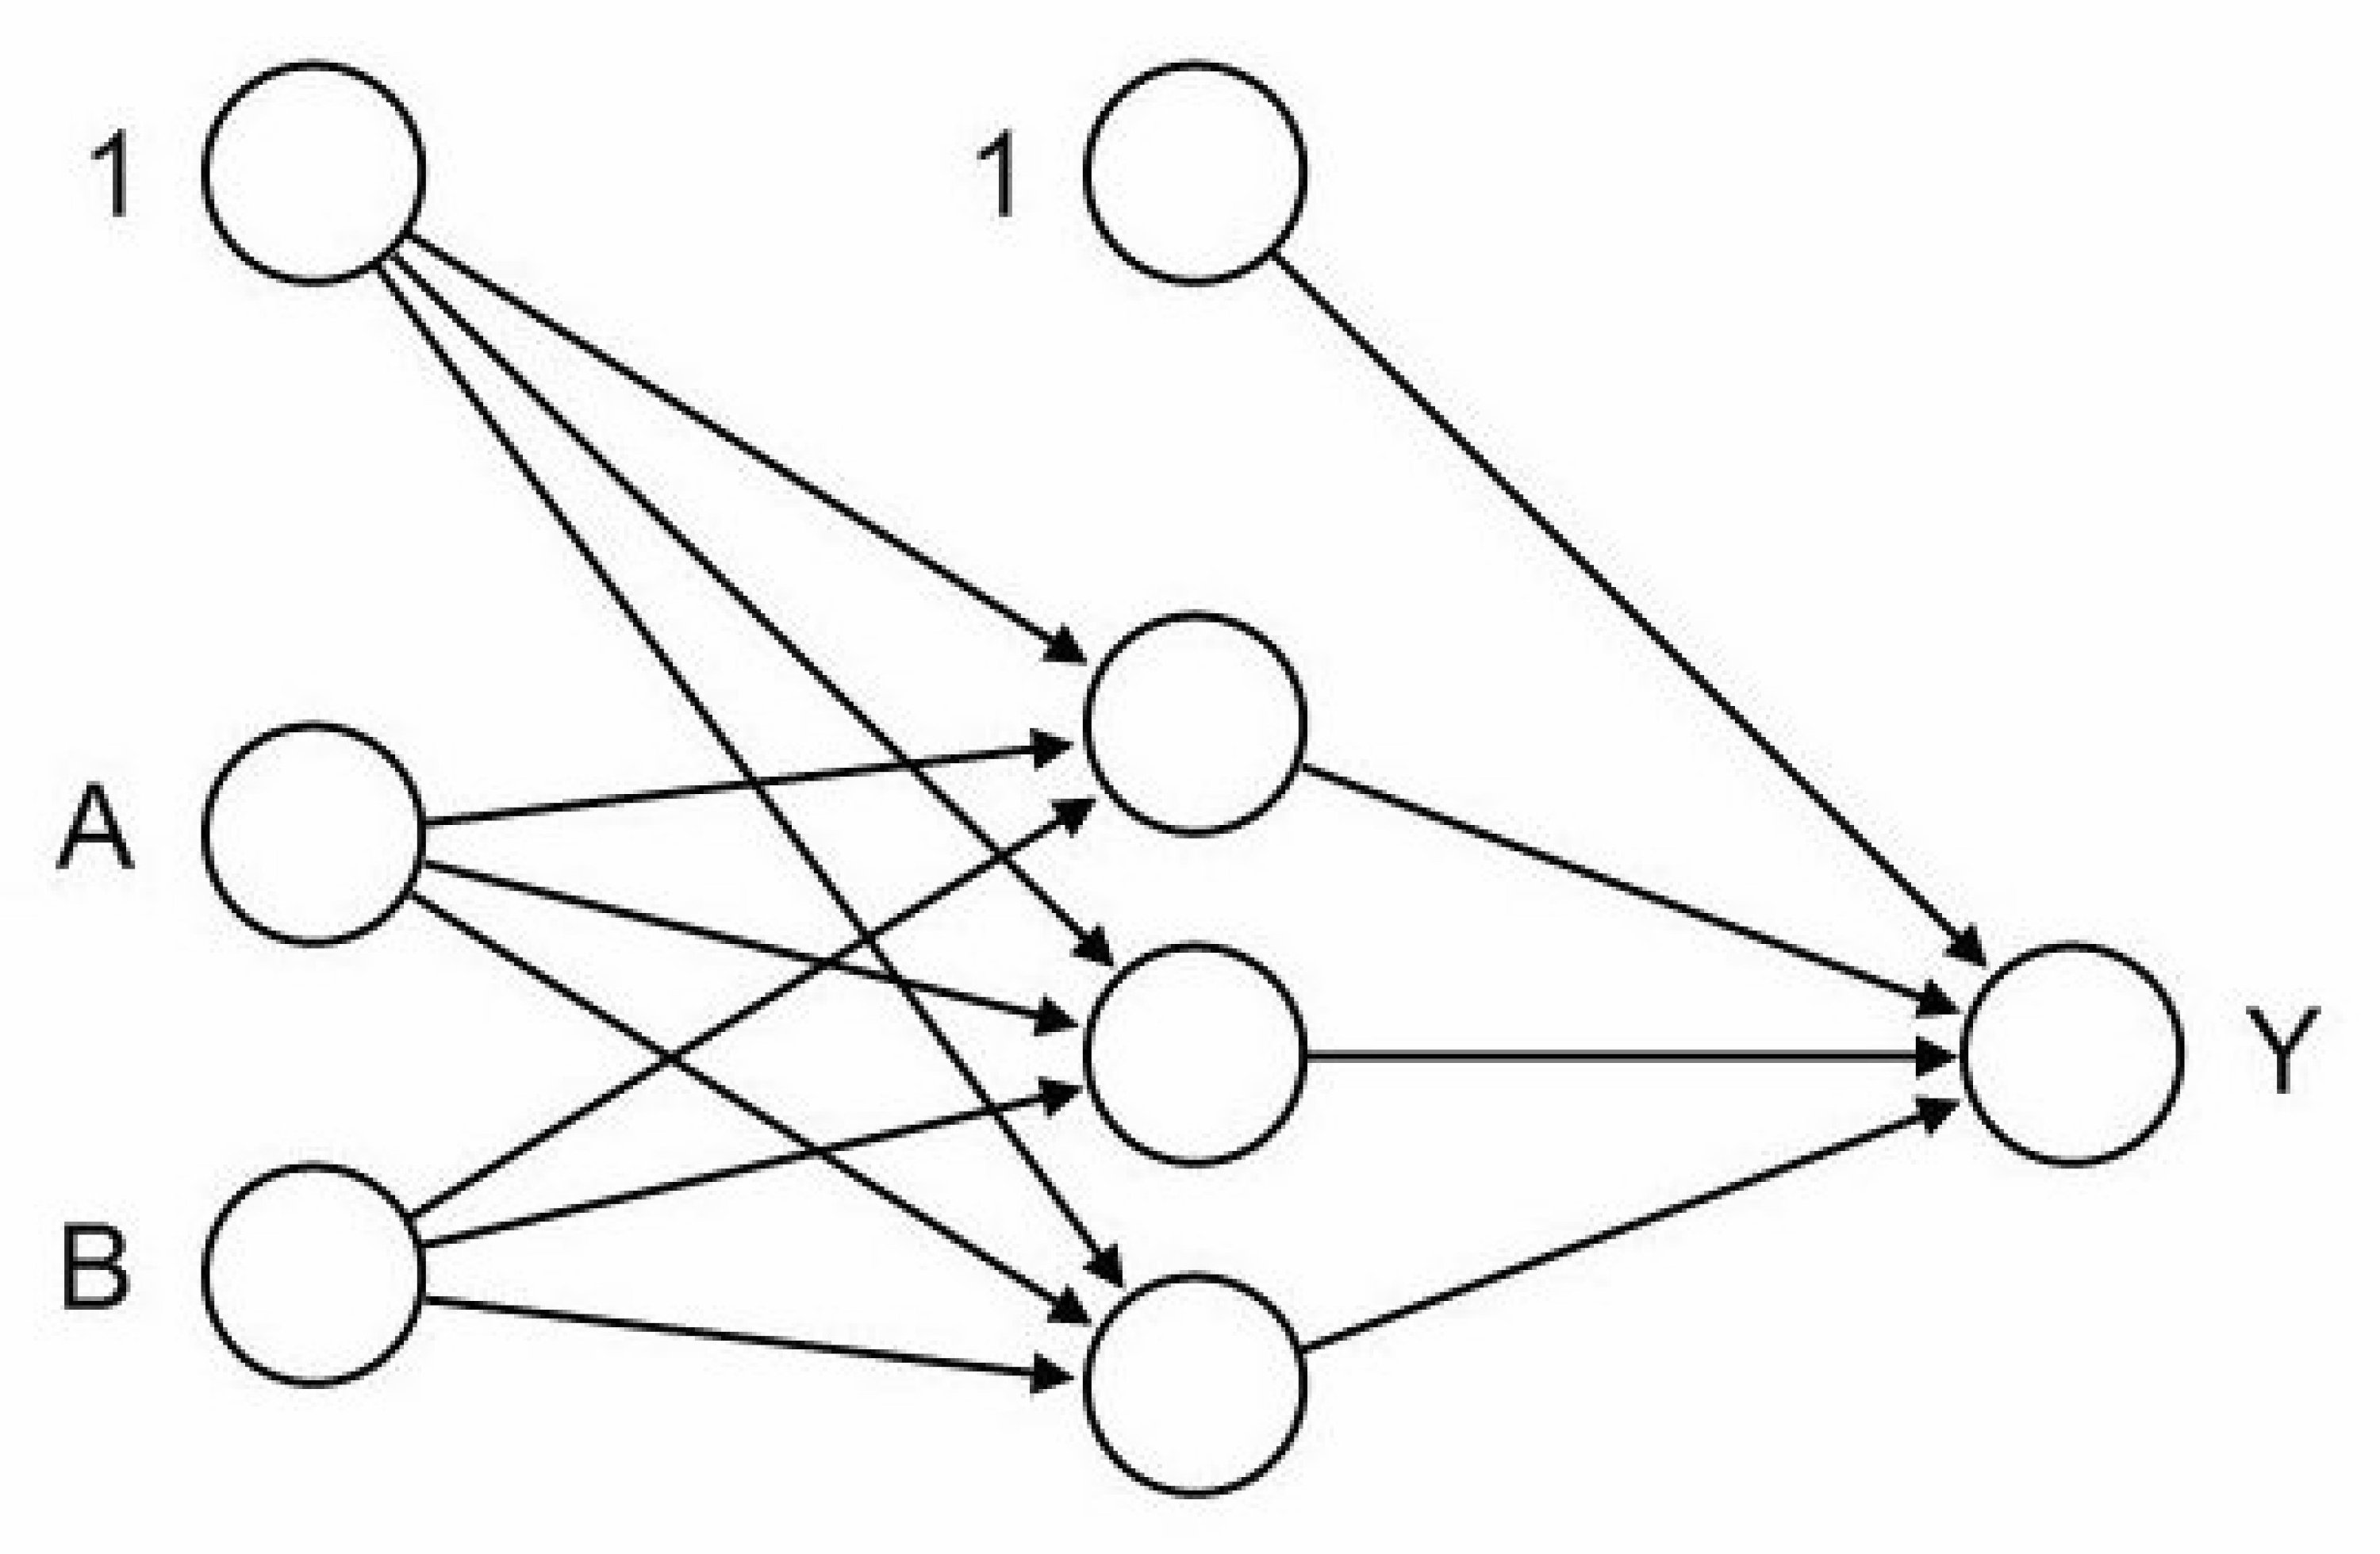
\includegraphics[width=0.7\columnwidth]{graphics/neuralnet-MLP}
\par\end{centering}
\caption{{Single-layer MLP between inputs $A$ and $B,$ and output $Y.$
The digit $1$ denotes the constant term, or bias.}}
\end{figure}

\begin{itemize}
\item MLP with one hidden layer containing three neurons.
\item This neural network models the relationship between two explanatory
variables, $A$ and $B,$ and the scalar response variable $Y.$ 
\item A weight, $w,$ is attributed to each synapse, indicating the effect
of the corresponding neuron, as if all the data were passing through
the NN as signals. 
\item The signals are then analyzed by 
\begin{itemize}
\item the \textcolor{magenta}{integration function} that combines all entering
signals,
\item then by the \textcolor{magenta}{activation function }that transforms
the output of each neuron.
\end{itemize}
\end{itemize}

\foilhead{MLP 3: model formulation }
\begin{itemize}
\item The \textcolor{magenta}{simplest MLP} consists of an input layer with
$n$ covariates, and an output layer with a single output neuron,
\[
o(x)=f\left(w_{0}+\sum_{i=1}^{n}w_{i}x_{i}\right)=f\left(w_{0}+\mathbf{w}^{\T}\mathbf{x}\right),
\]
where $w_{0}$ is the \textcolor{magenta}{intercept}, $\mathbf{w}=(w_{1},\ldots,w_{n})$
is the vector of synapse \textcolor{magenta}{weights}, and $\mathbf{x}=(x_{1},\ldots,x_{n})$
is the vector of all the \textcolor{magenta}{explanatory} variables. 
\item To increase the flexibility of the model, \textcolor{magenta}{hidden
layers} can then be added. In fact it can be proved that a single
layer is sufficient for modeling any piecewise continuous function. 
\item For a model with one hidden layer of $J$ hidden neurons, we have
\begin{align*}
o(x) & =f\left(w_{0}+\sum_{j=1}^{J}w_{j}\cdot f\left(w_{0j}+\sum_{i=1}^{n}w_{ij}x_{i}\right)\right)\\
 & =f\left(w_{0}+\sum_{j=1}^{J}w_{j}\cdot f\left(w_{0j}+\mathbf{w}_{j}^{T}\mathbf{x}\right)\right),
\end{align*}
where $w_{0}$ is the intercept of the output neuron, $w_{0j}$ the
intercept of the $j$-th hidden neuron. 
\item Formally, all the hidden neurons and the output neuron calculate 
\[
f\left(g(z_{0},z_{1},\ldots,z_{k})\right)=f\left(g(\mathbf{z})\right)
\]
from the outputs of all the preceding neurons, $z_{0},z_{1},\ldots,z_{k}$
where $g\,\colon\mathbb{R}^{k+1}\rightarrow\mathbb{R}$ is the \textcolor{magenta}{integration}
function and $f\,\colon\mathbb{R}\rightarrow\mathbb{R}$ is the \textcolor{magenta}{activation}
function. 
\item Note that the neuron $z_{0}=1$ is the constant neuron attached to
the intercept. 
\item The \textcolor{magenta}{integration} function is often defined by
\[
g(\mathbf{z})=w_{0}+\sum_{i=1}^{k}w_{i}z_{i}=w_{0}+\mathbf{w}^{T}\mathbf{z}.
\]
\item The \textcolor{magenta}{activation} function, $f,$ is a bounded,
non-decreasing, nonlinear and differentiable function that should
be chosen in relation with the response variable. 
\begin{itemize}
\item For example, the \textcolor{magenta}{logistic} function is recommended
for variables with a binary response.
\end{itemize}
\end{itemize}

\foilhead{The \texttt{\textcolor{blue}{neuralnet}} package of R }
\begin{itemize}
\item Implements training of <<\textcolor{magenta}{Multi-Layer Perceptrons}>>
(MLP) to learn the relation between explanatory variables (<<covariates>>)
and responses.
\item Uses a \textcolor{magenta}{backpropagation} method.
\item Can treat an arbitrary number of input and output variables. 
\item Can include an arbitrary number of hidden layers.
\end{itemize}

\foilhead{MLP 4: supervised learning}
\begin{itemize}
\item The \texttt{\textcolor{blue}{neuralnet}} function of R uses supervised
learning algorithms where 
\begin{itemize}
\item the given output is compared with the computed value, 
\item then the weights are adapted with respect to the comparison results. 
\item The weights are initialized by Gaussian random values. 
\end{itemize}
\item Then the iterative training process is:
\begin{itemize}
\item The NN calculates an output $o(\mathbf{x})$ for the given inputs,
$\mathbf{x},$ and the actual weights;
\item if the learning process is not finished, the predicted output, $o,$
will differ from the observed output, $y.$ 
\item The error is measured by a function, $E,$ as the\textcolor{magenta}{{}
sum of squared errors} (SSE)\index{neural networks (NN)!sum of squared errors (SSE)}
\[
E=\frac{1}{2}\sum_{l=1}^{L}\sum_{h=1}^{H}\left(o_{lh}-y_{lh}\right)^{2}
\]
or the\textcolor{magenta}{{} cross-entropy} \index{neural networks (NN)!cross-entropy}
\[
E=-\sum_{l=1}^{L}\sum_{h=1}^{H}\left(y_{lh}\log(o_{lh})+(1-y_{lh})\log(1-o_{lh})\right),
\]
where $l$ is the index of the observations and $h$ that of the observation
nodes. 
\end{itemize}
\item The weights are adjusted according to the rules of the learning algorithm---usually
stochastic gradient\index{optimization!stochastic gradient} plus
backpropagation (SGD + backprop).
\end{itemize}

\foilhead{MLP 5 : use of \texttt{\textcolor{blue}{neuralnet}} - arguments}
\begin{itemize}
\item There are two essential arguments: 
\begin{itemize}
\item (1) the \textcolor{magenta}{formula} (of type \texttt{lm}): \texttt{\textcolor{blue}{response
\textasciitilde{} covariate}}, 
\item (2) a \textcolor{magenta}{dataset} that contains the covariates and
the responses. 
\end{itemize}
\item All the other arguments have default values. 
\item Training: 
\begin{itemize}
\item We can define the \textcolor{magenta}{numbers} of hidden layers and
neurons per layer. 
\item The default value is a single hidden layer. 
\end{itemize}
\item The most important arguments are: 
\begin{itemize}
\item \texttt{\textcolor{blue}{formula}}: a symbolic description of the
model to be fitted (no default value). 
\item \texttt{\textcolor{blue}{data}}: a dataframe that contains the data
specified in \texttt{formula}. 
\item \texttt{\textcolor{blue}{hidden}}: a vector defining the number of
hidden layers and the hidden neurons in each layer (by default $1$). 
\item \texttt{\textcolor{blue}{threshold}}: a numerical value defining the
stopping criterion for the partial derivatives of $E$ with respect
to $w_{i}$ (by default $0.01$). 
\item \texttt{\textcolor{blue}{rep}}: number of repetitions for the learning
process (by default $1$). 
\item \texttt{\textcolor{blue}{err.fct}}: differentiable error function,
\texttt{sse} (sum squared error) or \texttt{ce} (cross entropy error)---by
default \texttt{sse}. 
\item \texttt{\textcolor{blue}{act.fct}}: differentiable activation function,
\texttt{logistic} or \texttt{tanh}---by default \texttt{logistic}. 
\item \texttt{\textcolor{blue}{linear.output}}: logical value that determines
if \texttt{act.fct} should not be applied to the output neurons---by
default \texttt{TRUE}. 
\item \texttt{\textcolor{blue}{likelihood}}: logical value equal to \texttt{TRUE}
if the error function is the negative log-likelihood function that
computes the information criteria of Akaike (AIC)\index{information criteria!AIC statistic}
and Bayes (BIC)\index{information criteria!BIC statistic}---by default
\texttt{FALSE}. 
\end{itemize}
\item Note that if the response variable is \textbf{binary}, one must choose: 
\begin{itemize}
\item activation function: \textcolor{magenta}{logistic}, 
\item error function: \textcolor{magenta}{cross entropy}, 
\item \texttt{linear.output} must be \texttt{FALSE} so that the output is
mapped by the activation function into the interval $\left[0,1\right].$ 
\end{itemize}
\end{itemize}

\foilhead{MLP 6: use of \texttt{\textcolor{blue}{neuralnet}} - outputs}
\begin{itemize}
\item Basic information on the learning process and the trained network
are stored in the direct output of the call to \texttt{neuralnet}. 
\item \texttt{\textcolor{blue}{net.result}}\texttt{ } is a list that contains
the output of the NN for each replication. 
\item \texttt{\textcolor{blue}{weights}} is a list that contains the fitted
weights. 
\item \texttt{\textcolor{blue}{result.matrix}} is a matrix that contains
the error, threshold, number of steps, AIC and BIC. 
\end{itemize}

\foilhead{MLP 6: use of \texttt{\textcolor{blue}{neuralnet}} - visualization}
\begin{itemize}
\item The results of the training can be visualized by
\begin{itemize}
\item \texttt{> plot(nn)}
\end{itemize}
\end{itemize}
\begin{figure}
\centering{}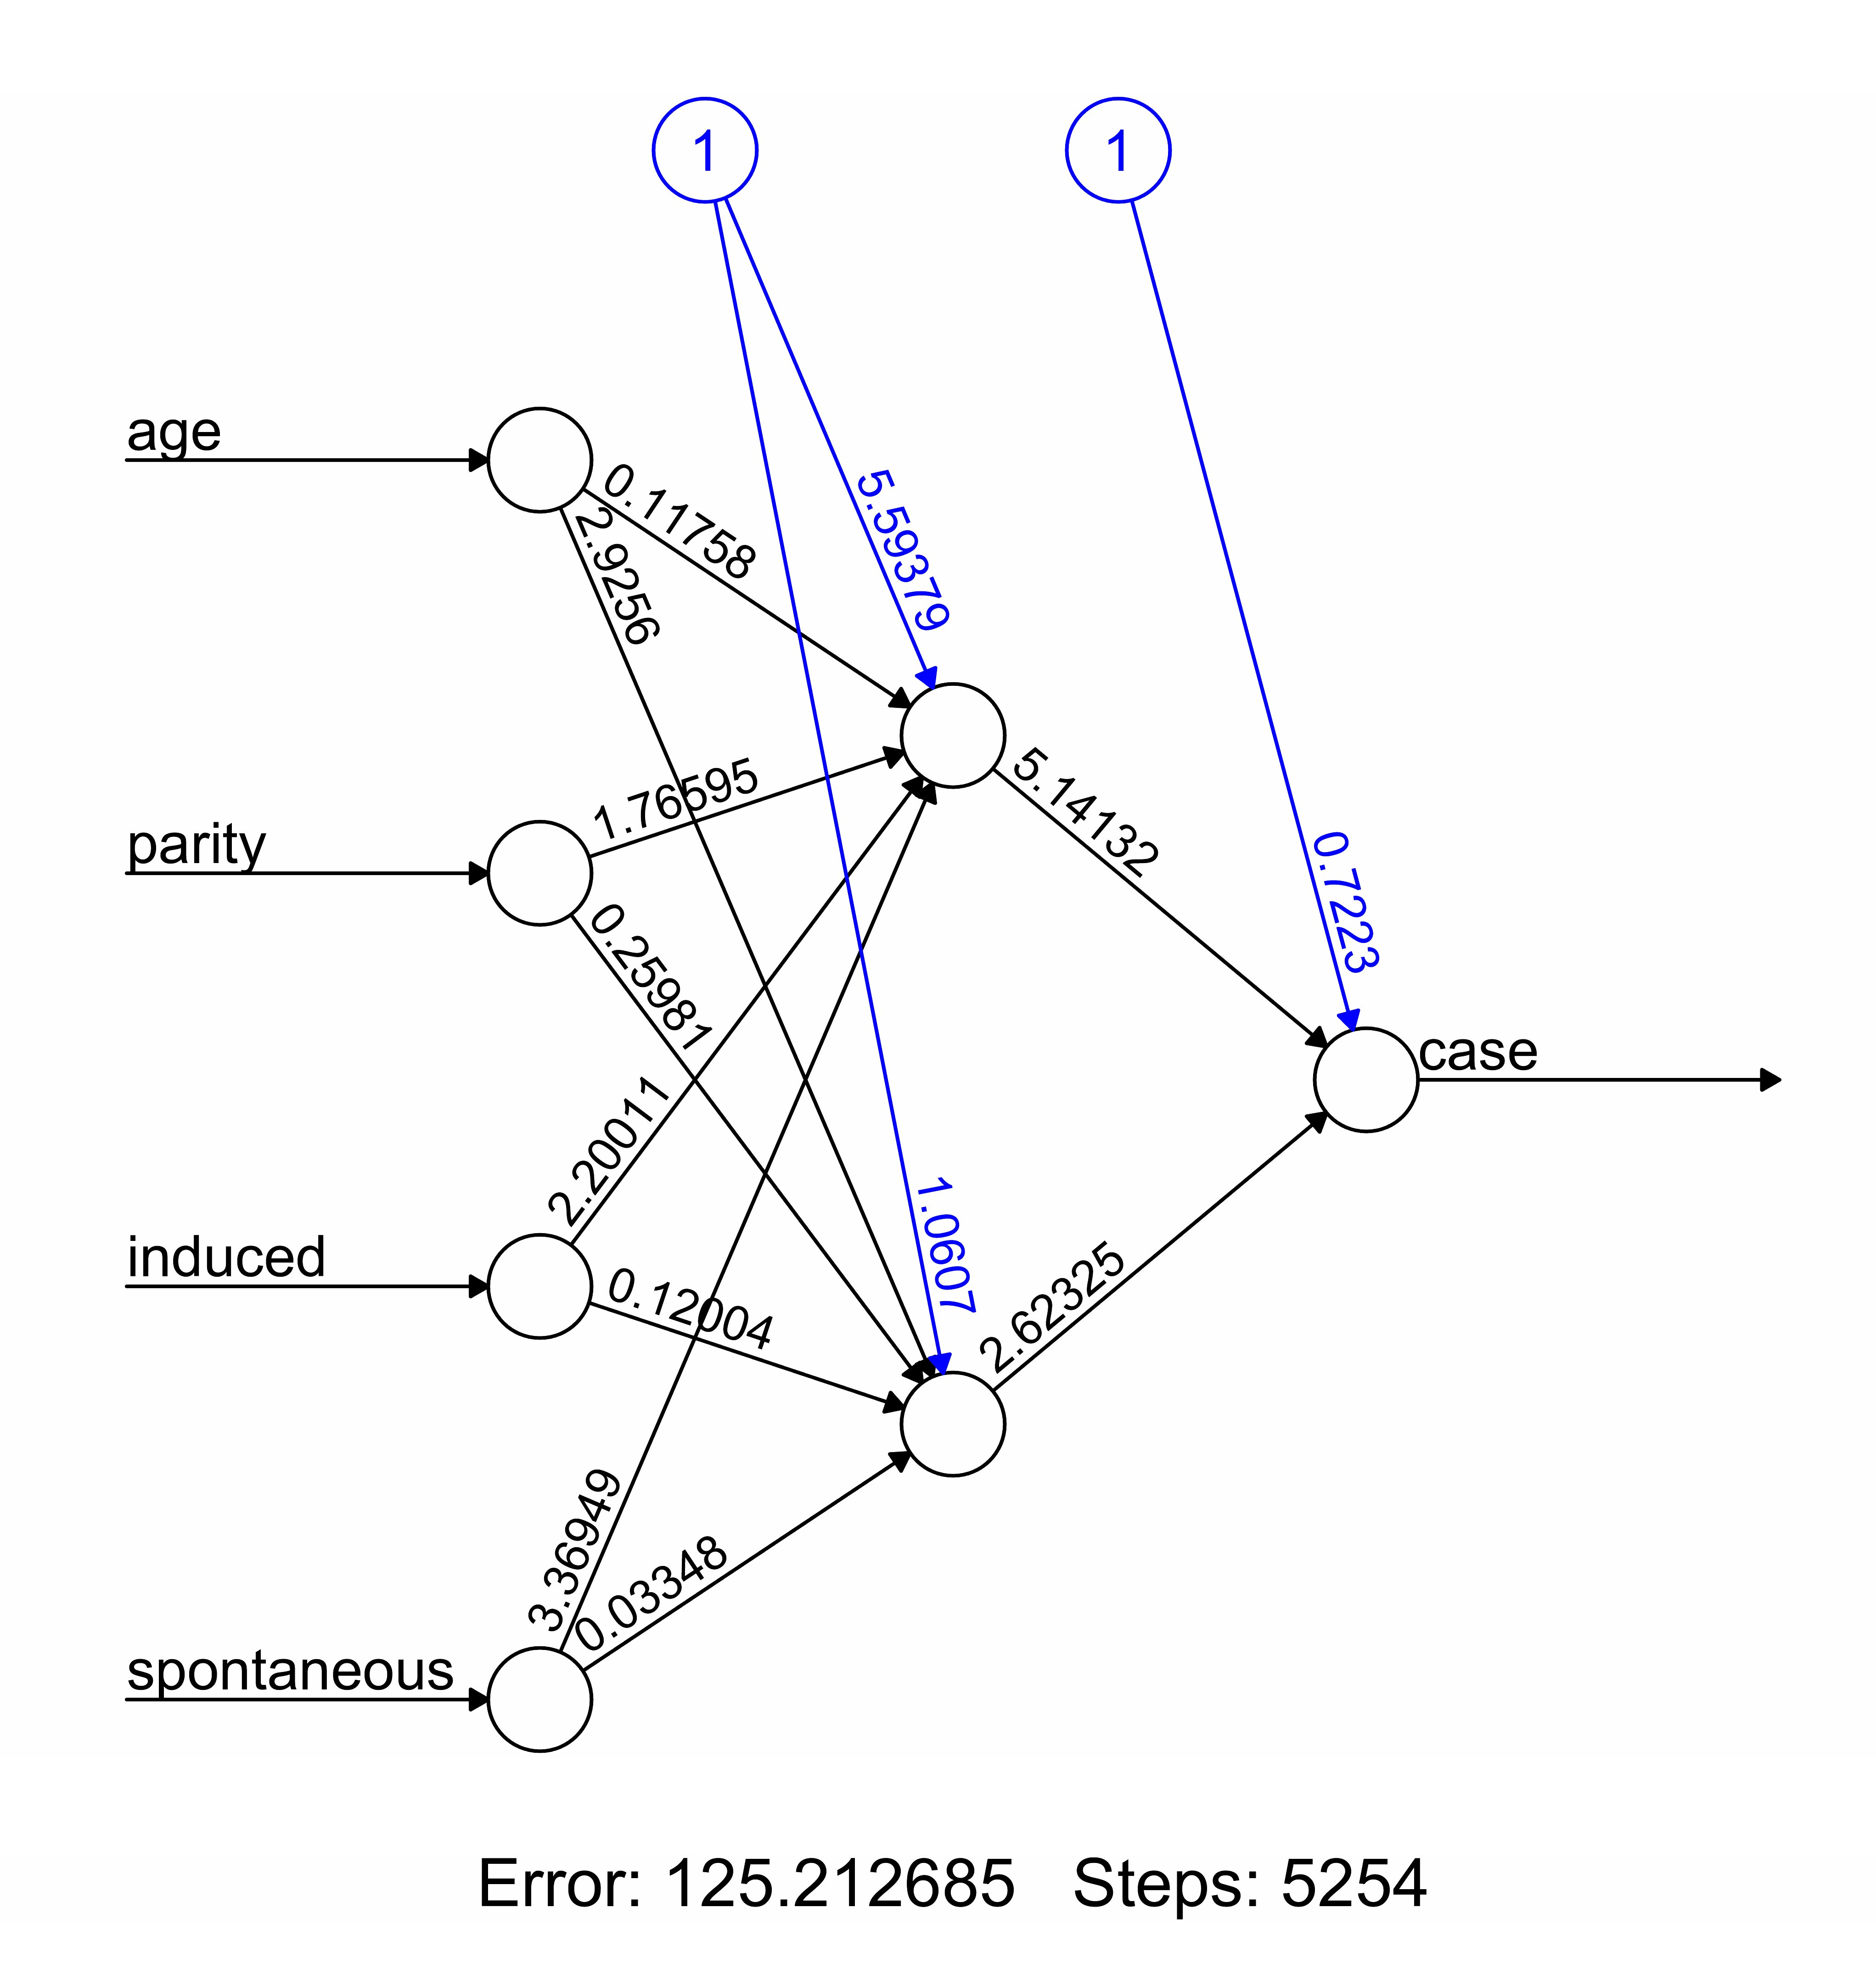
\includegraphics[width=0.7\columnwidth]{graphics/neuralnet-MLP-plot}
\end{figure}

\begin{itemize}
\item The plot shows:
\begin{itemize}
\item the topological structure of the network, 
\item the synaptic weights after training, 
\item all the intercepts, 
\item the global error and the number of steps required for convergence. 
\end{itemize}
\end{itemize}

\foilhead{Examples}
\begin{enumerate}
\item Toy 2D classification : \url{https://cs.stanford.edu/people/karpathy/convnetjs/demo/classify2d.html}
\item Synthetic data (simple example) : \texttt{\textcolor{blue}{nnet-squares.html}}
\item Stock exchange data: \texttt{\textcolor{blue}{nnet-dividendes.html}}
\item Fuel consumption data: \texttt{\textcolor{blue}{nnet-essence.html}}
\item Wine data: \texttt{\textcolor{blue}{nnet-MLP-wine.html.}}
\end{enumerate}

\foilhead{References}
\begin{enumerate}
\item I. Goodfellow, Y. Bengio, A. Courville. \emph{Deep Learning.} MIT
Press. 2016. \texttt{\textcolor{blue}{}}~\\
\texttt{\textcolor{blue}{}}~\\
\texttt{\textcolor{blue}{http://www.deeplearningbook.org}}%{\url{http://www.deeplearningbook.org}}
\item Rachel Schutt and Cathy O\textquoteright Neil. \emph{Doing Data Science.}
O'Reilly. 2014.
\end{enumerate}

\end{document}
